% Chapter 2

\chapter{Network Comparison and Conclusions} % Main chapter title

\label{Chapter3} % For referencing the chapter elsewhere, use \ref{Chapter1} 

%----------------------------------------------------------------------------------------


%----------------------------------------------------------------------------------------

\section{Network Comparison}

Until now, three different networks has been studied but no comparison has been established between them. In this section qualitative and quantitative results from the best scheme of each network will be compared and possible reasons of the results will be elaborated.\\

\begin{table}[h!]
  \begin{center}
    
    \begin{tabular}{|c|c|c|c|} % <-- Changed to S here.
    \hline
      \textbf{} & \textbf{ ICNet} & \textbf{SegNet} & \textbf{Stacked Hourglass} \\
      \hline
      Number of trainable variables & 6.743.733 & 5.904.921 & 14.804.962\\     
      \hline
    \end{tabular}
    \caption{Number of trainable parameters for each of the networks (best performing version}
    \label{final:table3}
  \end{center}
\end{table}

In Table \ref{final:table1} results regarding the three main metrics (mIoU, F1 and Accuracy) in the test set are shown. As seen the best performing one is the stacked hourglass. There are two important comments to be made: one reason to this outstanding performance compared to the other two networks could be the fact that the network is defined for the human body. Nevertheless, as a second comment, it could be argued that in this study the number of parameters has not been equalized and then, as the stacked hourglass is bigger than the other two it is natural that it has a better performance. The same problem could be stated between ICNet and SegNet but only with regards the number of parameters. In Table \ref{final:table3} the number of parameters of each of the best performing networks can be checked. As seen the Stacked Hourglass has more than double parameters compared to ICNet.\\
 
\begin{table}[h!]
  \begin{center}
    
    \begin{tabular}{|c|c|c|c|} % <-- Changed to S here.
      \textbf{Architecture} & \textbf{mIoU ($\%$)} & \textbf{Accuracy ($\%$)} & \textbf{F1 ($\%$)} \\
      \hline
      ICNet & 45.14 & 95.76 & 89.73\\
      \hline
      SegNet & 33.59 & 94.62  & 44.32 \\  
      \hline
      Stacked Hourglass & 55.32 & 97.02 & 93.07\\
    \end{tabular}
    \caption{Performance results on test set for the best performing scheme of each of the three networks selected.}
    \label{final:table1}
  \end{center}
\end{table}

Regarding accuracy per class, results can be observed in Table \ref{final:table2}. As seen both ICNet and Segnet show similar results with poorer results in low pixel area classes. On the contrary, the Stacked Hourglass has a more balanced result with a certain and significant improvement in the classes with low number of pixels. Nevertheless, the same problem of size commented before can be associated to this results. Hence the good balancing of the class accuracy results of the Stacked Hourglass network could be due to its size/complexity or its affinity towards human body data.\\


\begin{table}[h!]
  \begin{center}
    \resizebox{\textwidth}{!}{
    \begin{tabular}{|c|c|c|c|c|c|c|c|c|c|c|c|c|c|c|c|c|c|c|c|c|c|c|} % <-- Changed to S here.
      \textbf{Architecture} & \textbf{All classes}&\textbf{Background} & \textbf{Head} & \textbf{Torso} & \textbf{U.Legs}& \textbf{L.Legs} & \textbf{Neck} & \textbf{Shoulder} & \textbf{U.Arms}& \textbf{L.Arms}& \textbf{Feets}& \textbf{Hands}& \textbf{Fingers} & \textbf{Toes}  \\
      ICNet & 95.7 & 89.3 & 60.6 & 76.7 & 78.5 & 64.9 & 65.9 &10.6 & 41.9 & 64.5 & 59.8 & 43.1 & 33.9 & 42.5 \\
      \hline
      SegNet & 94.3 & 99.8 & 68.6 & 63.3 & 56.7 & 45.0 & 30.4 & 32.3 & 41.7 & 23.5 & 22.8 & 10.9 & 6.0 & 4.7\\
      \hline
      Stacked Hourglass  & 98.4 & 99.7 & 74.5 & 76.4 & 79.9 & 78.2 & 64.8 & 44.7 & 49.4 & 52.2 & 48.6 & 41.0 & 45.3 & 55.4\\
 	      \end{tabular}}
    \caption{Performance results on test dataset regarding accuracy per class for the best performing schemes of each of the three structures}
    \label{final:table2}
  \end{center}
\end{table}


In Figure \ref{final:inference} qualitative results of the best performing schemes of each network can be observed. As seen the best quality is shown by Stacked Hourglass. This could be due to the continuous refinement of the output in the pipeline. The poorest results are shown by SegNet Basic. This could be due to the low number of parameters or to the network configuration. Since it has only one top-down bottom-up process refinement is not carried out. Also, in the upsampling process information is lost, although skip connections help to avoid this loss. Nevertheless, since only indexes, and not full maps are stored, the recovering is not complete (although it speeds up the process). Regarding ICNet the results are pretty good but not as good as in Stacked Hourglass. This could be done to the use of the full resolution branch only when doing inference. This causes loss of precision but enhances inference speed.\\



\begin{figure}
\centering
\begin{subfigure}{.19\textwidth}
\centering
  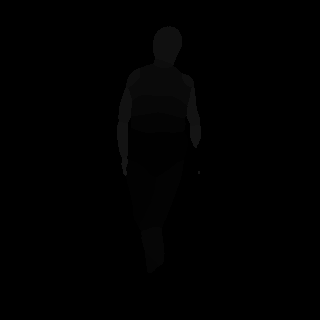
\includegraphics[scale=0.3]{ung_104_36_c0011_segm_7.png}
\end{subfigure}
\begin{subfigure}{.19\textwidth}
  \centering
  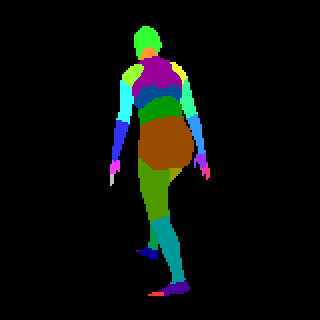
\includegraphics[scale=0.3]{36_10_c0019_segm_10.png}
\end{subfigure}
\begin{subfigure}{.19\textwidth}
  \centering
  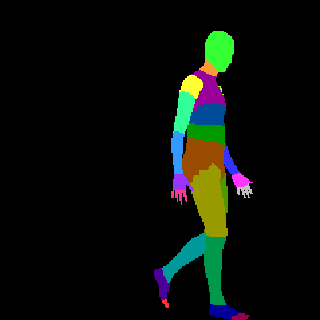
\includegraphics[scale=0.3]{40_02_c0011_segm_19.png}
\end{subfigure}
\begin{subfigure}{.19\textwidth}
  \centering
  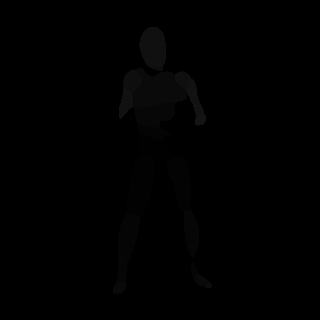
\includegraphics[scale=0.3]{104_52_c0002_segm_64.png}\\
\end{subfigure}\\
\begin{subfigure}{.198\textwidth}
\centering
  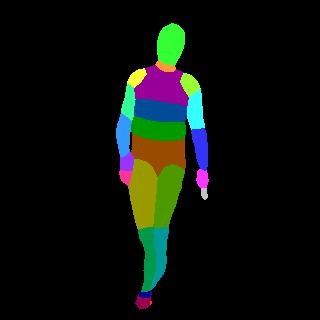
\includegraphics[scale=0.295]{ung_104_36_c0011_7_ice.jpg}
\end{subfigure}%
\begin{subfigure}{.19\textwidth}
  \centering
  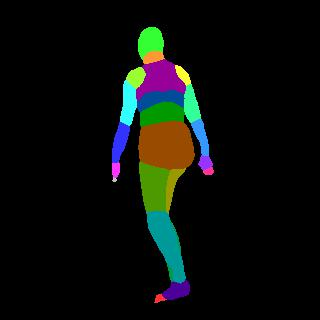
\includegraphics[scale=0.295]{36_10_c0019_10_ice.jpg}
\end{subfigure}
\begin{subfigure}{.19\textwidth}
  \centering
  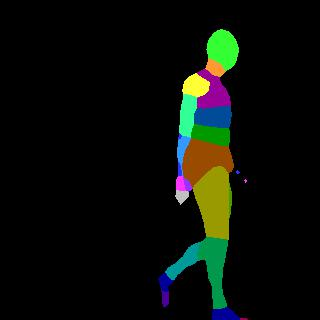
\includegraphics[scale=0.295]{40_02_c0011_19_ice.jpg}
\end{subfigure}
\begin{subfigure}{.189\textwidth}
  \centering
  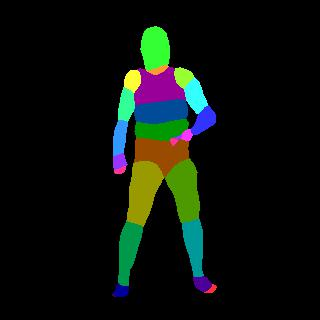
\includegraphics[scale=0.296]{104_52_c0002_64_ice.jpg}
\end{subfigure}\\
\begin{subfigure}{.19\textwidth}
\centering
  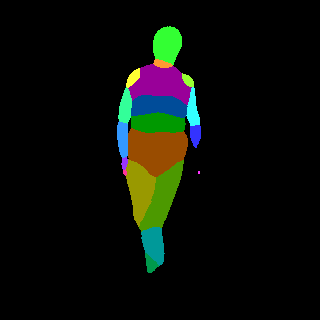
\includegraphics[scale=0.3]{ung_104_36_c0011_segm_7_seg.png}
\end{subfigure}
\begin{subfigure}{.19\textwidth}
  \centering
  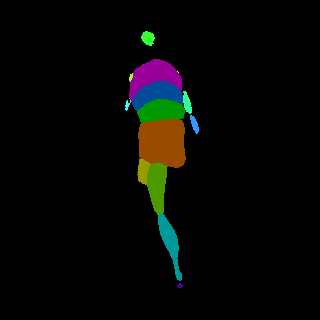
\includegraphics[scale=0.3]{36_10_c0019_segm_10_seg.png}
\end{subfigure}
\begin{subfigure}{.19\textwidth}
  \centering
  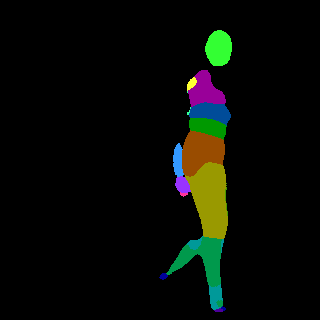
\includegraphics[scale=0.3]{40_02_c0011_segm_19_seg.png}
\end{subfigure}
\begin{subfigure}{.19\textwidth}
  \centering
  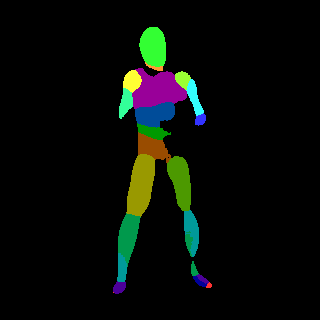
\includegraphics[scale=0.3]{104_52_c0002_segm_64_seg.png}\\
\end{subfigure}\\
\begin{subfigure}{.198\textwidth}
\centering
  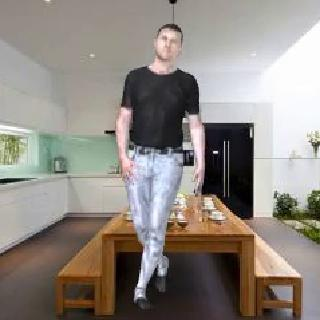
\includegraphics[scale=0.295]{ung_104_36_c0011_7.jpg}
\end{subfigure}%
\begin{subfigure}{.19\textwidth}
  \centering
  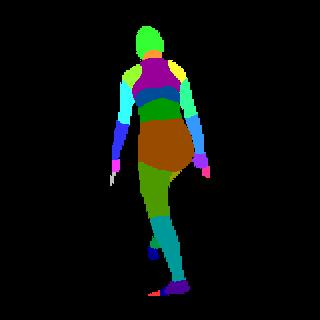
\includegraphics[scale=0.295]{36_10_c0019_10.jpg}
\end{subfigure}
\begin{subfigure}{.19\textwidth}
  \centering
  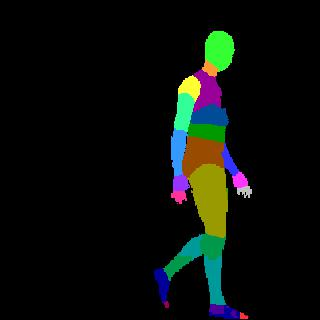
\includegraphics[scale=0.295]{40_02_c0011_19.jpg}
\end{subfigure}
\begin{subfigure}{.189\textwidth}
  \centering
  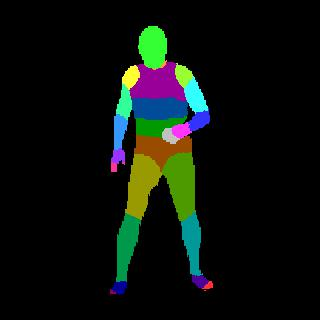
\includegraphics[scale=0.296]{104_52_c0002_64.jpg}
\end{subfigure}

\caption{First row: ground truth examples.  Second row: inference results with best ICNet model. Third row: inference results with best Segnet model. Fourth row: inference results with best Hourglass model.}
\label{final:inference}
\end{figure}

 



\section{Conclusions}
 	   
In this study we have analyzed three different structures which have as a main component convolution layers. ICNet focuses on different resolution samples of the same image through different branches to speed up inference but maintaining accuracy. SegNet, in our case SegNet Basic, uses an encoder decoder network with skip connections to avoid on-memory overloading and fast inference. And finally, Stacked Hourglass, which through its use of consecutive modules and residual components enables the refining process of the output produced. \\

In two different configurations of experiments, one for generally purposed networks and another for specific purposed networks, we have tried to improve the results obtained with these networks with regards the chosen dataset: SURREAL. Unfortunately, in almost none of them the results has been positive. In the first set of networks, the only positive results has been the doubling of filters in Segnet but not any other network configuration. In the second part, none of the new configurations have improved the results.\\

As a main drawback of this study it can be emphasized the fact that the networks were not in size/complexity equality: they differed in the number of parameters. Hence, this includes a bias to the study. Nevertheless, this  has not prevented us to satisfactorily obtain results from the three and be able to establish the differences in performance and use.\\

Regarding the future work that could be done, there are two main points: one is to include more networks to the study to make it more diverse and representative, and the second is to include the previously named problem, that is, configure the networks so, more or less, all have the same size or are similar in terms of complexity.\\

As a conclusion, this study has been centered on the examination and performance of three different fully convolutional networks applied to the SURREAL dataset. As a matter of fact, the Stacked Hourglass network has proven to be far better than the other two networks, although it has not been possible to establish clearly the reason: being size, structure definition or data type affinity. The results on the modifications of the networks have not been positive but have enabled the student to acquire a certain level, regarding both programming skills and field concepts, to carry on further and deeper studies. \\